\chapter{Proverb 27}

\begin{figure}
  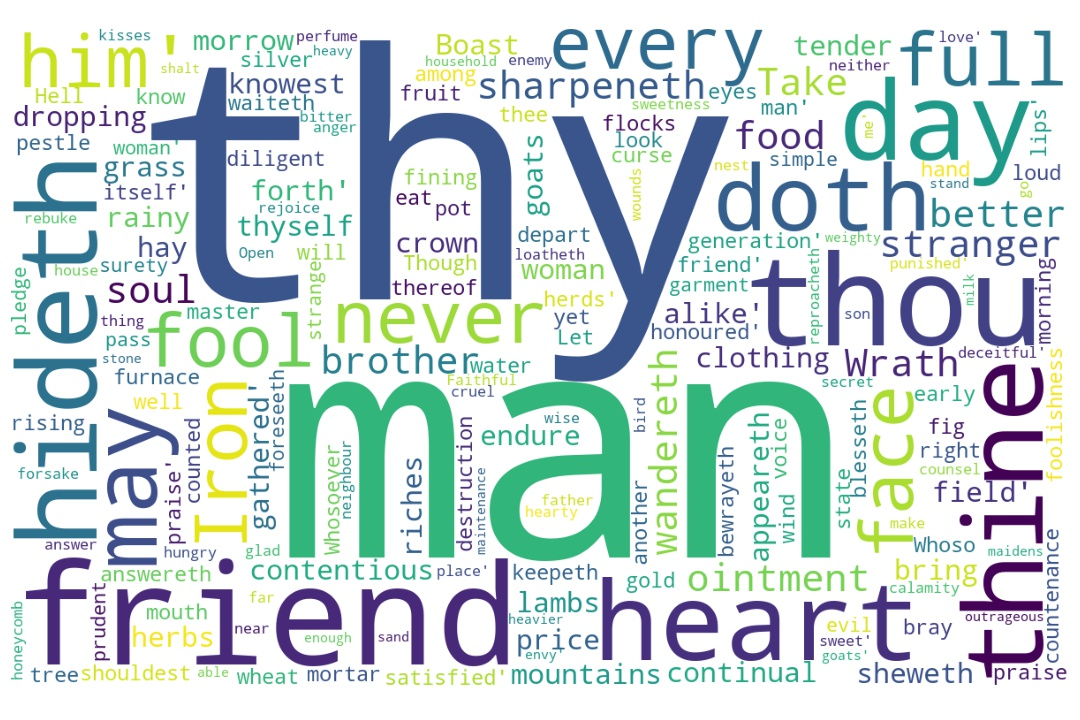
\includegraphics[width=\linewidth]{20OT-Proverbs/Proverb27-WordCloud.jpg}
  \caption{Proverb 27 Word Cloud}
  \label{fig:Proverb 27 word Cloud}
\end{figure}

\marginpar{\scriptsize \centering \fcolorbox{bone}{lime}{\textbf{A FAITHFUL MAN IN ACTION}}\\ (Proverb 27:1--27) \begin{compactenum}[I.][8]
    \item He is \textbf{Praised} by Others \index[scripture]{Proverbs!Pro 27:02}(Pro 27:2) 
    \item He is \textbf{Persevering} \index[scripture]{Proverbs!Pro 27:08}(Pro 27:8) 
    \item He is \textbf{Prudent} \index[scripture]{Proverbs!Pro 27:12}(Pro 27:12) 
    \item He is \textbf{Protected} \index[scripture]{Proverbs!Pro 27:12}(Pro 27:12) 
    \item He is \textbf{Principled} \index[scripture]{Proverbs!Pro 27:17}(Pro 27:17) 
    \item He is \textbf{Purified} \index[scripture]{Proverbs!Pro 27:21}(Pro 27:21) 
    \item He is \textbf{Provided for} \index[scripture]{Proverbs!Pro 27:27}(Pro 27:27) 
\end{compactenum}}


% counsel [9], continuance [17], countenance, contention [15], curse, calamity [10], conceipt, cruelty [4]


\footnote{\textcolor[cmyk]{0.99998,1,0,0}{\hyperlink{TOC}{Return to end of Table of Contents.}}}\footnote{\href{https://www.audioverse.org/english/audiobibles/books/ENGKJV/O/Prov/1}{\textcolor[cmyk]{0.99998,1,0,0}{Proverbs Audio}}}\textcolor[cmyk]{0.99998,1,0,0}{Boast not thyself of to morrow; for thou knowest not what a day may bring forth.}\footnote{\textbf{James 4:14} -  Whereas ye know not what shall be on the morrow. For what is your life? It is even a vapour, that appeareth for a little time, and then vanisheth away.}
[2] \textcolor[cmyk]{0.99998,1,0,0}{Let another man \fcolorbox{bone}{lime}{praise} thee, and not thine own mouth; a stranger, and not thine own lips.}
[3] \textcolor[cmyk]{0.99998,1,0,0}{A stone \emph{is} heavy, and the sand weighty; but a fool's wrath \emph{is} heavier than them both.}\footnote{\textbf{Proverb 12:16} - A fool’s wrath is presently known: but a prudent man covereth shame.}
[4] \textcolor[cmyk]{0.99998,1,0,0}{Wrath \emph{is} cruel, and anger \emph{is} outrageous; but who \emph{is} able to stand before envy?}
[5] \textcolor[cmyk]{0.99998,1,0,0}{Open rebuke \emph{is} better than secret love.}
[6] \textcolor[cmyk]{0.99998,1,0,0}{Faithful \emph{are} the wounds of a friend; but the kisses of an enemy \emph{are} deceitful.}\footnote{\textbf{2 Samuel 20:9-10} - And Joab said to Amasa, Art thou in health, my brother? And Joab took Amasa by the beard with the right hand to kiss him. [10] But Amasa took no heed to the sword that was in Joab’s hand: so he smote him therewith in the fifth rib, and shed out his bowels to the ground, and struck him not again; and he died. So Joab and Abishai his brother pursued after Sheba the son of Bichri.}\footnote{\textbf{Matthew 26:48-50} - Now he that betrayed him gave them a sign, saying, Whomsoever I shall kiss, that same is he: hold him fast. [49] And forthwith he came to Jesus, and said, Hail, master; and kissed him. [50] And Jesus said unto him, \textcolor{myRed}{Friend, wherefore art thou come?} Then came they, and laid hands on Jesus, and took him.}
[7] \textcolor[cmyk]{0.99998,1,0,0}{The full soul loatheth an honeycomb; but to the hungry soul every bitter thing is sweet.}
[8] \textcolor[cmyk]{0.99998,1,0,0}{As a bird that \fcolorbox{bone}{lime}{wandereth} from her nest, so \emph{is} a man that \fcolorbox{bone}{lime}{wandereth} from his place.}
[9] \textcolor[cmyk]{0.99998,1,0,0}{Ointment and perfume rejoice the heart: so \emph{doth} the sweetness of a man's friend by hearty counsel.}
[10] \textcolor[cmyk]{0.99998,1,0,0}{Thine own friend, and thy father's friend, forsake not; neither go into thy brother's house in the day of thy calamity: \emph{for} better \emph{is} a neighbour \emph{that} \emph{is} near than a brother far off.}
[11] \textcolor[cmyk]{0.99998,1,0,0}{My son, be wise, and make my heart glad, that I may answer him that reproacheth me.}
[12] \textcolor[cmyk]{0.99998,1,0,0}{A \fcolorbox{bone}{lime}{prudent} \emph{man} foreseeth the evil, \emph{and} \fcolorbox{bone}{lime}{hideth himself}; \emph{but} the simple pass on, \emph{and} are punished.}
[13] \textcolor[cmyk]{0.99998,1,0,0}{Take his garment that is surety for a stranger, and take a pledge of him for a strange woman.}
[14] \textcolor[cmyk]{0.99998,1,0,0}{He that blesseth his friend with a loud voice, rising early in the morning, it shall be counted a curse to him.}
[15] \textcolor[cmyk]{0.99998,1,0,0}{A continual dropping in a very rainy day and a contentious woman are alike.}
[16] \textcolor[cmyk]{0.99998,1,0,0}{Whosoever hideth her hideth the wind, and the ointment of his right hand, \emph{which} bewrayeth \emph{itself}.}
[17] \textcolor[cmyk]{0.99998,1,0,0}{Iron \fcolorbox{bone}{lime}{sharpeneth} iron; so a man \fcolorbox{bone}{lime}{sharpeneth} the countenance of his friend.}
[18] \textcolor[cmyk]{0.99998,1,0,0}{Whoso keepeth the fig tree shall eat the fruit thereof: so he that waiteth on his master shall be honoured.}
[19] \textcolor[cmyk]{0.99998,1,0,0}{As in water face \emph{answereth} to face, so the heart of man to man.}
[20] \textcolor[cmyk]{0.99998,1,0,0}{Hell and destruction are never full; so the eyes of man are never satisfied.}
[21] \textcolor[cmyk]{0.99998,1,0,0}{\emph{As} the \fcolorbox{bone}{lime}{fining pot} for silver, and the furnace for gold; so \emph{is} a man to his praise.}
[22] \textcolor[cmyk]{0.99998,1,0,0}{Though thou shouldest bray a fool in a mortar among wheat with a pestle, \emph{yet} will not his foolishness depart from him.}
[23] \textcolor[cmyk]{0.99998,1,0,0}{Be thou diligent to know the state of thy flocks, \emph{and} look well to thy herds.}
[24] \textcolor[cmyk]{0.99998,1,0,0}{For riches \emph{are} not for ever: and doth the crown \emph{endure} to every generation?}
[25] \textcolor[cmyk]{0.99998,1,0,0}{The hay appeareth, and the tender grass sheweth itself, and herbs of the mountains are gathered.}
[26] \textcolor[cmyk]{0.99998,1,0,0}{The lambs \emph{are} for thy clothing, and the goats \emph{are} the price of the field.}
[27] \textcolor[cmyk]{0.99998,1,0,0}{And \emph{thou} \emph{shalt} \emph{have} goats' milk \fcolorbox{bone}{lime}{enough} for thy food, for the food of thy household, and \emph{for} the maintenance for thy maidens.}


